% !TeX root = ../main.tex
% !TeX encoding = UTF-8
% !TeX spellcheck = none
\subsection{Hyperparameter Sensitivity Analysis}\label{sec:exp-hyperparameters}

\hpupdated{We conducted one-factor-at-a-time validation experiments on Chengdu to examine how SERR gating capacity, BCMS representation capacity, and the initial values of two residual pathways affect prediction error. The SERR gating hidden dimension and the BCMS internal representation dimension each took values in \(\{8,16,32,64,128\}\). Both \(\alpha_0\) and \(\beta_0\) took values in \(\{0,0.001,0.01,0.05,0.1\}\). They specify the initial values of the learnable residual parameters defined in Sections~\ref{sec:serr} and~\ref{sec:bcms}, respectively, and these parameters continue to update during training. The reference configuration was \((32,32,0,0)\), as used in the main comparison experiments. We changed one parameter at a time while keeping all other settings fixed. \editorialupdated{Bold tick labels indicate the reference configuration, and the minimum within each group was determined from unrounded results.} Training, checkpoint selection, and validation aggregation followed Sections~\ref{sec:exp-implementation} and~\ref{sec:exp-datasets}.}

\hpupdated{We first constructed the model with the reference configuration and replaced the gating or BCMS module only when its dimension differed from 32. Residual initial values were assigned directly to the learnable parameters. Neither training nor validation used additional splitting into microbatches.}

\hpupdated{All four parameters produced only small changes in joint validation error within the tested ranges (Figure~\ref{fig:hyperparameter-joint}). We calculated each group's relative range as the difference between its maximum and minimum errors divided by the error of the reference configuration. Across the four groups, this range was below 0.15\% for joint MAE and below 0.35\% for joint RMSE.}

\begin{figure}[!htbp]
  \centering
  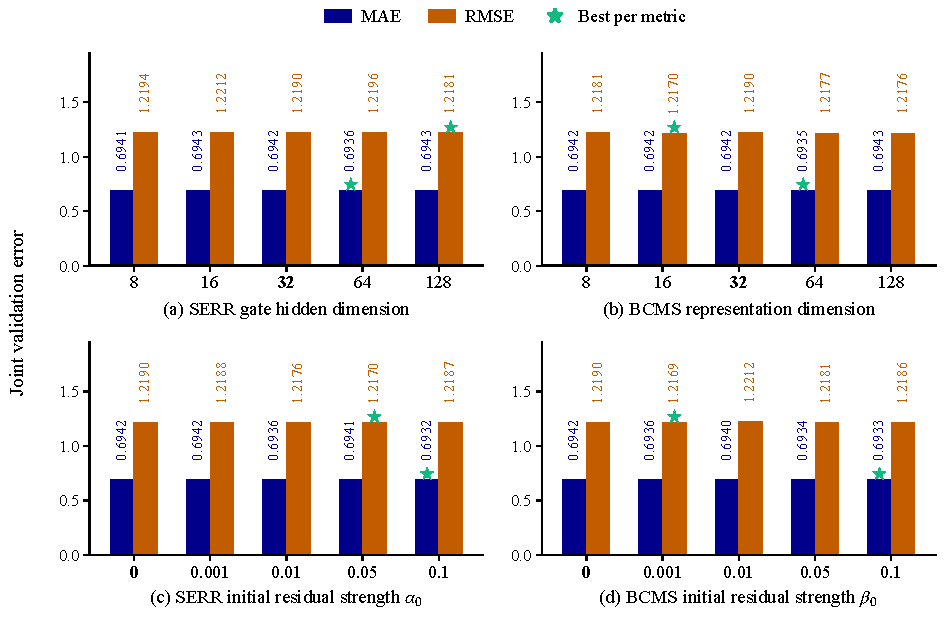
\includegraphics[width=\linewidth]{figures/hyperparameter-joint.pdf}
  \caption{\editorialupdated{Hyperparameter sensitivity of joint validation metrics on the Chengdu dataset.}}
  \label{fig:hyperparameter-joint}
\end{figure}

\hpupdated{Increasing the hidden dimension did not consistently reduce error, and the lowest joint MAE and RMSE occurred at different dimensions. The best positive initial values of the residual parameters provided only small improvements over zero initialization. The two metrics likewise did not share a single optimal initial value.}

\hpupdated{Figure~\ref{fig:hyperparameter-flow} presents the complete results for each flow channel. The small changes in joint error also included different responses across channels. For the SERR gating dimension, inflow MAE was lowest at 64, whereas outflow MAE was lowest at 8. Thus, the two flow channels responded differently to gating capacity.}

\begin{figure}[!htbp]
  \centering
  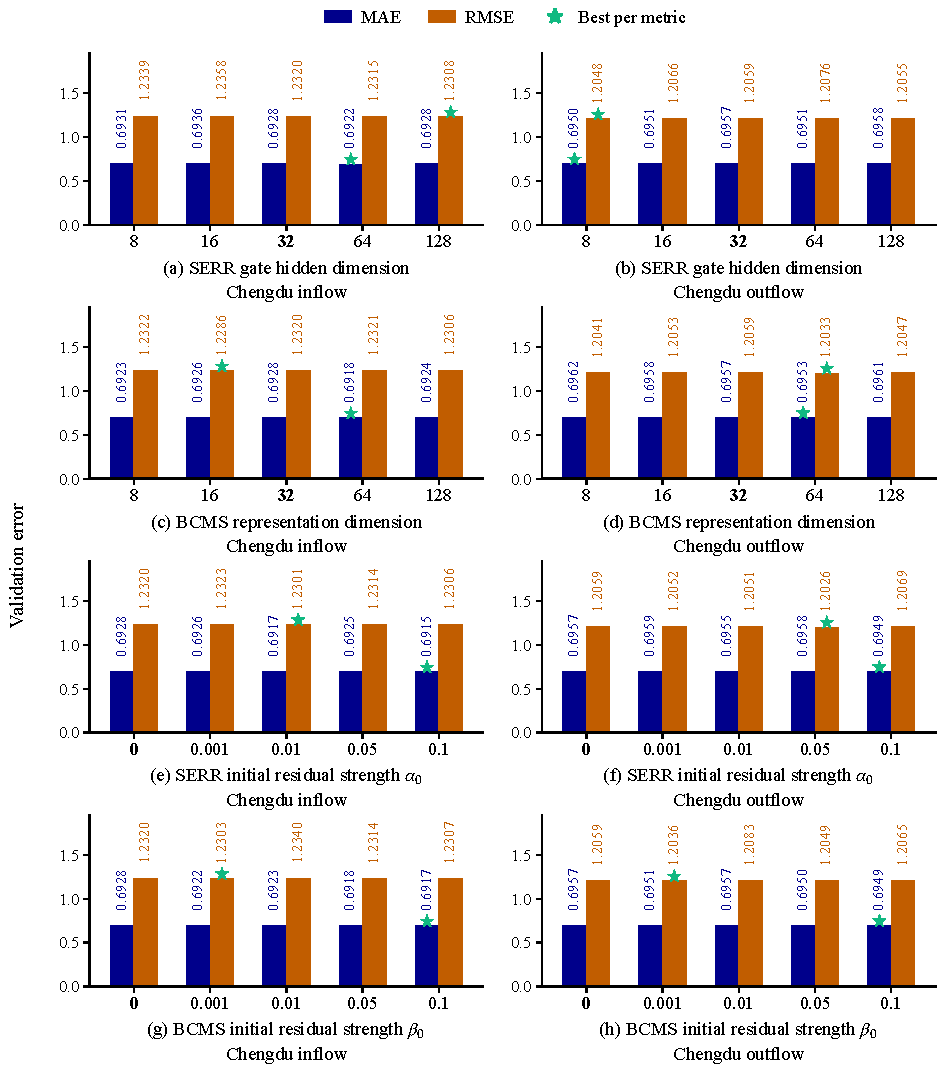
\includegraphics[width=\linewidth]{figures/hyperparameter-flow.pdf}
  \caption{\editorialupdated{Hyperparameter sensitivity for inflow and outflow on the Chengdu dataset.}}
  \label{fig:hyperparameter-flow}
\end{figure}
\FloatBarrier
